\lstdefinestyle{myLatex} { 
  language=[LaTeX]TeX
  , texcsstyle=*\bf\color{blue} 
  , basicstyle=\ttfamily
  , numbers=none
  , breaklines=true
  , commentstyle=\color{red}
  %, otherkeywords={$, \{, \}, \[, \]} 
  %, frame=lines 
  , xleftmargin=30pt          % linker Abstand vom Rand (framesep+framrule)
  , tabsize=2
  %, caption=LaTeX example
}

\chapter{Wie ich Newton Polygone zeichne}
Der code
\begin{lstlisting}[style=myLatex]
\newcommand{\myNewtonPlot}[6]{
  \draw[color=black,thick] #2;
  \foreach \pos in #1 { \fill[blue,opacity=.2] (-.5,#5) rectangle \pos; }
  \draw[->] (-.5,0) -- (#3+.7,0);
  \draw[->] (0,#4-.2) -- (0,#5+.2);
  \draw (1,0) -- (1,-.2);
  \draw (0,1) -- (-.2,1);
  \foreach \pos in #1 { \node[draw,circle,inner sep=1.5pt,fill=white] at \pos {}; }
  \node [below right] at (#3,#5/2) {#6};
}
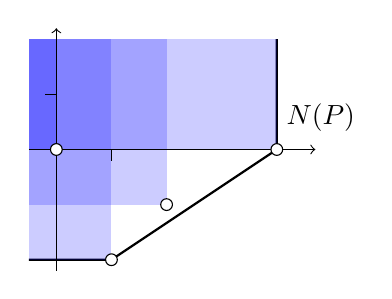
\begin{tikzpicture}[scale=0.7]
\def\myPoints{{(0,0)}, {(1,-2)}, {(2,-1)}, {(4,0)}}
\def\myPath{(-.5,-2) -- (1,-2) -- (4,0) -- (4,2)}
\myNewtonPlot{\myPoints}{\myPath}{4}{-2}{2}{$N(P)$}
\end{tikzpicture}
\end{lstlisting}

ergibt

\begin{center}
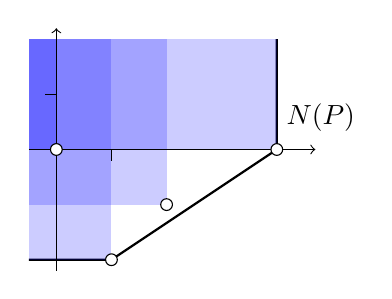
\begin{tikzpicture}[scale=0.7]
\def\myPoints{{(0,0)}, {(1,-2)}, {(2,-1)}, {(4,0)}}
\def\myPath{(-.5,-2) -- (1,-2) -- (4,0) -- (4,2)}
\myNewtonPlot{\myPoints}{\myPath}{4}{-2}{2}{$N(P)$}
\end{tikzpicture}
\end{center}

% vim: set ft=tex :
